\chapter{Tanimoto Random Features}
\label{chapter:trf}

This chapter presents an algorithm to produce random feature
approximations for the Tanimoto kernel,
which is a popular kernel in cheminformatics
(introduced in \S\ref{sec:background:mol-kernels}).
It was published as a conference paper
in NeurIPS 2023 \citep{tripp2023tanimoto}.
This conference paper was jointly written with
Prof.\@ Sergio Bacallado (Cambridge Statistical Laboratory),
my supervisor José Miguel Hernández-Lobato,
and Miguel's postdoc Sukriti Singh.
The initial idea for this algorithm was proposed by Sergio,
and I helped refine the ideas and conducted experiments.
The manuscript was primarily written by myself and Sergio,
although all authors contributed.

\section{Motivation}
\label{sec:trf:motivation}

The methods presented in chapters \ref{chapter:lso} and \ref{chapter:adkf}
use deep-kernel Gaussian process models to predict molecular properties.
However, in one way or another both of these methods require large amounts of data
to fit the parameters of the underlying neural network.
With a small amount of data,
perhaps the best one can do is use a simple classical cheminformatics kernel,
such as a kernel on molecular fingerprints (e.g.\@ Tanimoto kernel)
or any one of many previously proposed graph kernels (see \S\ref{sec:background:mol-kernels}).

Unfortunately, as graph kernels are less widely used than kernels in $\R^n$,
there are fewer methods which build on top of them.
In particular, there are fewer approximations to these kernels
which would allow GPs to scale to large datasets.
Inducing point methods (\S\ref{sec:background:approx-gp-inference})
are in principle agnostic to the kernel used,
but in practice the inducing points are often chosen using gradient-based optimisation,
which is not applicable when the inducing points are discrete objects like graphs.
Random feature methods are specific to a particular kernel,
and despite a lot of recent work on random features for kernels defined
\emph{on nodes within a graph} \citep{reid2023quasi,reid2024repelling,reid2024universal},
there is a lack of work on random features for kernels \emph{between graphs}.

This work stemmed from a handful of insights which allowed us to construct two kinds of random features for the Tanimoto kernel.
Combined with molecular fingerprint features (\S\ref{sec:background:fingerprints}),
this effectively creates a scalable graph kernel applicable to large molecular datasets.
Section~\ref{sec:trf:background} provides some background information,
and the main contributions of this chapter are presented in
sections~\ref{sec:minmax-rf} and \ref{sec:t-dp}.
Section~\ref{sec:trf:experiments} presents experiments.

\section{Background: Tanimoto kernel over \texorpdfstring{$\R^n$}{Rn}}
\label{sec:trf:background}

The Tanimoto kernel $T$ was defined over pairs of \emph{sets} in chapter~\ref{chapter:background} (equations~\ref{eqn:background:tanimoto-for-sets}
and \ref{eqn:background:tanimoto-for-multisets}).
However, because this chapter introduces several Tanimoto-like functions, we will introduce
some additional notation.
First, because this chapter is concerned with kernels over sets of vectors,
we write $x_i$ to refer to the $i$th element of a vector and $x^{(i)}$ to denote the $i$th vector in a list.
Second, note that if $S$ is a subset of a finite set $\Omega$,
$S$ can be represented as a binary \emph{indicator vector} $s\in\{0,1\}^{|\Omega|}$,
where $s_i=1$ if and only if the $i$th element of $\Omega$ is in $S$.
This also holds true for multi-sets, although in this case $s_i$ is the number of times the $i$th element appears in $S$.

Letting $d=|\Omega|$,
the Tanimoto kernel can be interpreted as a kernel over non-negative vectors in $\R^d_{\geq0}$:
\begin{equation}\label{eqn:minmax-kernel}
    T_{MM}(x, x') = \frac{\sum_i \min(x_i, x'_i)}{\sum_i \max(x_i, x'_i)}\,.
\end{equation}
This kernel is sometimes referred to as the ``Min-Max kernel'',
although in this chapter we will simply refer to it as $T_{MM}$.

The remainder of this chapter will simply consider the problem of defining random features
for the Tanimoto kernel over $\R^d_{\geq0}$,
rather than over fingerprint features specifically.
Although fingerprints are defined as sets of subgraphs in section~\ref{sec:background:fingerprints},
in practice these subgraphs are always hashed into $\mathbb{N}$,
thereby making the application of these random features to fingerprints straightforward.


\section{Low-variance random features for Tanimoto and MinMax kernels}\label{sec:minmax-rf}

Outside of chemistry, the Tanimoto coefficient has been widely used to measure the similarity
between text documents
and rank results in search engines.
To quickly find documents with high similarity to a user's query,
many prior works have studied random
\emph{hashes} for the Tanimoto coefficient,
i.e.\@ a family of random functions $h:\mathcal{X}\mapsto\{1,\ldots,K\}$ such that
\begin{equation}\label{eqn:random-hash-defn}
    \probability_h \left( h(x) = h(x') \right) = T_{MM}(x,x').
\end{equation}
Although initially these hashes were only applicable to binary inputs
\citep{broder1997resemblance,broder1998min,charikar2002similarity},
more recent work has produced efficient random hashes for arbitrary non-negative vectors
\citep{manasse2010consistent,ioffe2010improved,shrivastava2016simple}.
In this section we propose a novel family of low-variance random features for $T_{MM}$
(and by extension $T_{S}$) which is based on random hashes.

It is important to clarify that although the definition of random hashes in equation~\ref{eqn:random-hash-defn}
resembles the definition of random features in equation~\ref{eqn:random-feature-definition},
they are actually distinct.
Random hash functions output \emph{discrete} objects (typically an integer or tuple of integers)
whose probability of \emph{equality} is $T_{MM}$,
while random features must output \emph{vectors} in $\mathbb{R}^M$ whose expected \emph{inner product}
is $T_{MM}$.
If a random hash maps to $\{1,\ldots,K\}$,
a naive approach may be to use a $K$-dimensional indicator vector as a random feature.
Because hash equality is a binary outcome,
the variance of such random features would be $T_{MM}\left(1-T_{MM}\right)$.
Realistic hash functions like that of \citet{ioffe2010improved}
use $K\ge 10^3$,
implying a ``variance per feature'' of $\approx 10^2$,
which is undesirably high.

Our main insight is that low-variance scalar random features can be created
by using a random hash to \emph{index} a suitably distributed random vector.
In the following theorem, we show that a vector of i.i.d.\@ samples
from any distribution with the correct first and second moments
can be combined with random hashes to produce random features for $T_{MM}$.
\begin{theorem}\label{thm:general-minmax-rf}
    Let $h:\mathcal X \to \mathcal Y$ be a random hash for $T_{MM}$ satisfying equation~\ref{eqn:random-hash-defn}, with $|\mathcal Y|=K$. Furthermore, let $\xi$ be a random variable such that $\mathbb{E}[\xi]=0$ and $\mathbb{E}[\xi^2]=1$,
    and let $\Xi=[\xi_1,\ldots,\xi_K]$ be a vector of independent copies of $\xi$.
    Then the 1D random features 
    \begin{equation}\label{eqn:minmax-rf}
        \phi_{\Xi,h}(x)=\Xi_{h(x)}  
    \end{equation}
    estimate $T_{MM}$ without bias: 
    $\E_{\Xi,h}(\phi_{\Xi,h}(x)\cdot\phi_{\Xi,h}(x')) = T_{MM}(x,x')$,
    and with variance
    \begin{equation}\label{eqn:general-minmax-rf-variance}
    \mathbb{V}_{\Xi,h}\left[\phi_{\Xi,h}(x)\cdot \phi_{\Xi,h}(x')\right] = 1+T_{MM}(x,x')\left(E[\xi^4]-1-T_{MM}(x,x')\right) \ge 1-T_{MM}(x,x')^2.
    \end{equation}
    Furthermore, the lower bound is tight and achieved when $\xi$ is Rademacher distributed (i.e.\@ uniform in $\{-1,1\}$).
\end{theorem}

The proof is given in Appendix~\ref{apdx:minmax-rf-proof}. This theorem shows that Rademacher $\xi$ yields the smallest possible variance in the class of random features defined in \cref{eqn:minmax-rf}.

These random features have many desirable properties. First, unlike random features for many other kernels such as the Gaussian kernel \citep{liu2021random},
the variance does not depend on the dimension of the input data or norms of the input vectors.
Second, because these random features are 1-dimensional scalars,
$M$ independent random feature functions can be concatenated to produce $M$-dimensional random feature
vectors with variance at most $1/M$.
This suggests that as few as $\approx10^3$ random features could be used in practical problems.
Third, although each instance of $\Xi$ requires storing a $K$ dimensional random vector,
if $\xi$ is chosen to be Rademacher distributed, then each entry can be stored with a single bit,
requiring just $\approx 100$ kB of memory when $K=10^6$.

One disadvantage of these random features
is that they are not continuous or differentiable with respect to their inputs.
For applications such as Bayesian optimisation which require optimising over model inputs
this would create difficulties as gradient-based optimisation could no longer be done.
It was this disadvantage which motivated us to search for other random features,
leading to the discoveries in the following section.


\section{Tanimoto dot product kernel and its random features}\label{sec:t-dp}

\citet{ralaivola2005graph} gave a definition for the Tanimoto coefficient involving dot products:
\begin{equation}\label{eqn:tanidot-kernel}
    T_{DP}(x, x') = \frac{x\cdot x'}{\|x\|^2+\|x'\|^2-x\cdot x'},
\end{equation}
with $T_{DP}(x,x')=1$ when $x,x'=0$. It is easy to check that $T_{DP}(x,x')=T_{MM}(x,x')$ on binary vectors, which was used by \citet{ralaivola2005graph} to prove that $T_{DP}$ is a kernel on the space $\{0,1\}^d$, referencing prior work by \citet{gower1971general}.  However, $T_{DP}$ is not identical to $T_{MM}$ for general inputs $x,x'\in \R_{\ge 0}^d$. Here, we give the first proof that $T_{DP}$ is a positive definite function in $\R^d$ and thus, also a valid kernel in this space.

\begin{theorem}\label{thm:tdp-is-pd}
    For $x,x'\neq 0$ in $\R^d$, we have
    \begin{equation}\label{eqn:tanidot-power-series}
       T_{DP}(x,x')= \sum_{r=1}^\infty \left(x\cdot x'\right)^r \left(\|x\|^2+\|x'\|^2\right)^{-r},
    \end{equation}
    where the series is absolutely convergent. The function $T_{DP}$ is a positive definite kernel in $\R^d$.
\end{theorem}

It has been noticed previously that, unlike $1-T_{MM}$, the function $1-T_{DP}$ is \emph{not} a distance metric on non-binary inputs \citep{kosub2019note}. Indeed, when $d=1$, the inputs $\{1,2,4\}$   violate the triangle inequality. However, we can easily derive a distance metric from $T_{DP}$.

\begin{corollary}\label{thm:tdp-is-metric}
    $d_{DP}(x,x')=\sqrt{1-T_{DP}(x,x')}$ 
    corresponds to the RKHS norm of the function $\frac{1}{2}[T_{DP}(x,\cdot)-T_{DP}(x',\cdot)]$
    and is therefore a valid distance metric on $\mathbb{R}^d$.
\end{corollary}

Proofs are given in Appendix~\ref{apdx:tdp-is-pd-proof}. These results imply that $T_{DP}$, like $T_{MM}$, is an extension of the set-valued Tanimoto coefficient
(equation~\ref{eqn:background:tanimoto-for-sets})
to real vectors and can be used as a substitute for $T_{MM}$ in machine learning algorithms that require a kernel or distance metric. Unlike $T_{MM}$, the kernel $T_{DP}$
is differentiable everywhere with respect to its inputs.
It can also be computed in batches using matrix-matrix multiplication,
allowing for efficient vectorized computation.

We now consider producing a random features approximation to $T_{DP}$ for large-scale applications.
Motivated by the close relationship between $T_{DP}$ and $T_{MM}$,
one may be tempted to find a random hash for $T_{DP}$
and apply the techniques developed in section~\ref{sec:minmax-rf}.
Unfortunately, we are able to prove that this is not possible.
\begin{proposition}\label{no random hash for tdp}
    There exists no random hash function for $T_{DP}$ over non-binary vectors.
\end{proposition}
\begin{proof}
    \citet{charikar2002similarity} proved that if $s(x,x')$ is a similarity function
    for which there exists a random hash,
    then $1-s(x,x')$ must satisfy the triangle inequality (see their Lemma 1).
    Because $1-T_{DP}(x,x')$ does not satisfy the triangle inequality it follows by contradiction
    that there does not exist a random hash for $T_{DP}$.
\end{proof}

Therefore, producing random features for $T_{DP}$ will require another approach.
In the remainder of this section we present a framework to produce random features for $T_{DP}$ by directly approximating its power series
(equation~\ref{eqn:tanidot-power-series}).
We first describe a method to produce random features for $(\|x\|^2+\|x'\|^2)^{-r}$ (\S\ref{ssec:prefactor-rf}).
Then we describe how these features can be combined with existing random features for the polynomial kernel
to approximate $T_{DP}$'s truncated power series (\S\ref{sec:tdp-rf}--\ref{ssec:implementing tdp rf}).



\subsection{Random features for the ``prefactor'' \texorpdfstring{$\left(\|x\|^2+\|x'\|^2\right)^{-r}$}{}}\label{ssec:prefactor-rf}

In this section we present a random feature map for the positive definite kernel $\textstyle (x,x')\mapsto (\|x\|^2 + \|x'\|^2)^{-r}$,
which we will refer to as the \emph{prefactor}.
We defer all proofs to Appendix~\ref{apdx:prefactor-sketch}.
We begin with the following lemma, which defines scalar random features for the prefactor:

\begin{lemma}\label{scalar prefactor features lemma}
    If  $Z\sim\mathrm{Gamma}(s,c)$ (where $c$ is a \emph{rate} parameter), then
    \begin{align}
        \varphi_{r,Z}(x) = e^{(1/2-\|x\|^2)Z} Z^{(r-s)/2}\sqrt{c^{-s}e^{(c-1)Z}\Gamma(s)/{\Gamma(r)}}
    \end{align}
     is an unbiased scalar random feature for the prefactor $(\|x\|^2 + \|x'\|^2)^{-r}$
    for all $s,c>0$.
\end{lemma}
Although independent copies of $Z$ could be combined to form an $M$-dimensional sketch,
we instead propose to use a dependent point set $Z_1,\dots,Z_M$ where each element $Z_i$ has a Gamma$(s,c)$ distribution whilst maximally covering the real line. This is a well-established Quasi-Monte Carlo (QMC) technique which generally attains
lower variance. 
We define our $M$-dimensional QMC features in the following lemma:
\begin{lemma}\label{lemma:def QMC prefactor features}
     Let $\gamma_{s,c}$ be the inverse cumulative distribution function of a $\mathrm{Gamma}(s,c)$ random variable.
     Fix $M,r\in\mathbb{N}$, $u\in(0,1)$, $c,s>0$ and let $u_i = u + i/M - \lfloor u + i/M\rfloor$ for $i=1,\dots,M$.
     Define $\phi_{u,r}(x) = (\phi_{u,r,1}(x),\dots,\phi_{u,r,M}(x))$, where:
     \begin{equation}
         \phi_{u,r,i}(x) =\frac{1}{\sqrt M}\sqrt{\frac{c^{-s}\Gamma(s)}{\Gamma(r)} } e^{-(\|x\|^2-c/2)\gamma_{s,c}(u_i) }(\gamma_{s,c}(u_i))^{(r-s)/2}\ .
     \end{equation}
     If $u\sim\mathcal U(0,1)$ then $\phi_{u,r}(x)$ forms unbiased random features of the prefactor $(\|x\|^2 + \|x'\|^2)^{-r}$.
\end{lemma}
Although the random features are unbiased for all $s,c>0$, the value of these parameters will impact the error.
We show that if $s,c$ are suitably tuned, then the relative error can be bounded:
 \begin{lemma} \label{QMC error}
Let $x^{(1)},\dots,x^{(n)}\in \R^d$ with $\frac{\min_i \|x^{(i)}\|^2}{\max_i \|x^{(i)}\|^2} \ge \zeta$, and fix $u\in[0,1]$. Define the relative error
\begin{align}
    \label{error matrix}
E_{i,j} = \frac{   \phi_{u,r}(  x^{(i)} )\cdot \phi_{u,r}( x^{(j)} ) - (\| x^{(i)} \| ^2+ \| x^{(j)} \| ^2)^{-r} }{( \| x^{(i)} \| ^2+ \| x^{(j)} \| ^2)^{-r}} .
\end{align}
If $c = 2\zeta^2$, $s=r\zeta$, then 
for some constant $C$ independent of $r$
this error satisfies, 
\begin{align}
\max_{1\le i,j \le n} | E_{i,j}| \leq \frac{2}{M} \frac{\Gamma(r\zeta)\zeta^{-r\zeta}}{\Gamma(r)} (r/e)^{r(\zeta-1)} (1.3)^r \leq C (M\zeta)^{-1}.
\end{align}
\end{lemma}

Together, these lemmas suggest random features for the prefactor can be created
by first estimating $\zeta$ (the minimum ratio of norms of input vectors),
then using the random features from \Cref{lemma:def QMC prefactor features} with the
values of $s,c$ specified in \Cref{QMC error}.












\subsection{A framework to produce random features for \texorpdfstring{$T_{DP}$}{TDP}}
\label{sec:tdp-rf}

There are straightforward rules for producing random features for sums and products of kernels whose individual random features are known \citep[{\S}2.6.2]{duvenaud_2014}.
Random features for kernels $k_1,k_2$ can be \emph{concatenated} (denoted $\oplus$) to form random features for the sum kernel $k_1+k_2$,
while their \emph{tensor product}\footnote{
For two vectors $x\in\R^{d_1}$ and $y\in\R^{d_2}$, define the tensor product $x\otimes y = \text{vec}(xy^T) \in \R^{d_1d_2}$.
} (denoted $\otimes$)
forms random features for the product kernel $k_1\times k_2$.
Our strategy to produce features for $T_{DP}$ is
to combine random features for the ``prefactor'' (presented in \cref{ssec:prefactor-rf})
with random features for the polynomial kernel to produce random features for $T_{DP}$'s power series (equation~\ref{eqn:tanidot-power-series}) truncated at $R$ terms.

Fix $R\in\mathbb{N}$, and for $r=1,\ldots,R$, let $\phi_r$ be a $m_r$-dimensional random features map for the prefactor
$\textstyle (\|x\|^2 + \|x'\|^2)^{-r}$ and let $\psi_r$ be a $m'_r$-dimensional random features map for
$\left(x\cdot x'\right)^r$. The function:
\begin{equation}\label{naive tensor product rfs}
    \tilde\Phi_R(x) = \oplus_{r=1}^R \left[\phi_r(x) \otimes \psi_r(x)\right]
\end{equation}
is therefore a random feature estimate for $T_{DP}$'s power series, truncated at $R$ terms.
Unfortunately, these random features have dimension 
$M=\sum_{r=1}^R m_r m'_r$
which depends on the \emph{product} of the random features dimension of $\phi_r$ and $\psi_r$. Furthermore, the dimension $m_r'$ of the random features $\psi_r$ required to approximate the polynomial kernel $(x\cdot x')^r$ with good accuracy can scale poorly with $r$.
For even modest values of $m_r,m'_r$ the resulting value of $M$ will likely be prohibitively large.

To remedy this, we turn to recent works which propose powerful linear maps
to approximate tensor products
with a lower-dimensional vector.
Assuming $x^{(1)},y^{(1)}\in\R^{d_1}$ and $x^{(2)},y^{(2)}\in\R^{d_2}$,
these maps are effectively random matrices $\Pi\in \R^{m\times (d_1d_2)}$,
which exhibit a \emph{subspace embedding property} whereby $[\Pi(x^{(1)}\otimes x^{(2)})]\cdot[\Pi(y^{(1)}\otimes y^{(2)})]$ concentrates sharply around $(x^{(1)}\otimes x^{(2)})\cdot(y^{(1)}\otimes y^{(2)})$.
Critically, the product $\Pi(x^{(1)}\otimes x^{(2)})$ can be computed \emph{without} instantiating either matrix $\Pi$ or the tensor product $x^{(1)}\otimes x^{(2)}$.
Examples of such methods include
\textsc{TensorSketch} and \textsc{TensorSRHT}
\citep{pagh2013compressed,pham2013fast, ahle2020oblivious},
but for generality we will simply refer to these methods as \textsc{Sketch}.
Defining a series of sketches $\textsc{Sketch}_r:\R^{m_r}\times \R^{m'_r}\mapsto \R^{\tilde{m}_r}$
we can modify $\tilde\Phi_R$ from equation~\ref{naive tensor product rfs} into:
\begin{equation}\label{sketch tensor product rfs}
    \Phi_R(x) = \oplus_{r=1}^R \textsc{Sketch}_r\left[\phi_r(x),  \psi_r(x)\right]
\end{equation}
which has output dimension $M=\sum_{r=1}^R \tilde{m}_r$, i.e.\@ without any pathological dependencies on the dimensions of $\phi_r(x),\psi_r(x)$.


\subsection{Methods to correct the bias of Tanimoto dot product random features}
\label{apdx:bias-correction}

We begin by noting that when $x,x'\in\R_{\ge 0}^d$, $x\cdot x'\ge 0$, and therefore, the power series
\begin{align*}
T_{DP}(x,x')=\sum_{r=1}^\infty (x\cdot x')^r(\|x\|^2+\|x'\|^2)^{-r}
\end{align*}
is monotone. Therefore, if we use an unbiased sketch for the truncated series 
\begin{align*}
\sum_{r=1}^R (x\cdot x')^r(\|x\|^2+\|x'\|^2)^{-r}
\end{align*}
as the one constructed in Section \ref{sec:tdp-rf}, the final sketch will be biased \emph{downward}
for all $x,x'\in\R_{\ge 0}^d$, i.e.,
\begin{align*}
\E(\Phi(x)\cdot\Phi(x'))< T_{DP}(x,x') \ .
\end{align*}
Below we introduce two strategies to remedy this issue.

\subsubsection{Bias correction strategy 1: normalize the features}

As the kernel satisfies $T_{DP}(x,x)=1$ for all $x\in\R^d$, one possible correction is to \emph{normalize} the sketch to obtain
\begin{align*}
\tilde \Phi(x) = \frac{\Phi(x)}{\|\Phi(x)\|}.
\end{align*}
This remains an oblivious sketch, and ensures that the diagonal of the kernel matrix is estimated exactly, at the expense of possibly introducing some bias in off-diagonal elements of $K$.

\subsubsection{Bias correction strategy 2: sketch the residual}

To simplify the algebra,
let $t_{x,y}=\frac{x\cdot y}{\|x\|^2 + \|y\|^2}$.
The power series for $T_{DP}$ can then be re-written as:
\begin{align}
    T_{DP}(x,y) &= \sum_{r=1}^\infty \left(t_{x,y}\right)^r \nonumber\\
    &= \sum_{r=1}^{R} \left(t_{x,y}\right)^r + \left(t_{x,y}\right)^{R+1} + \sum_{r=R+2}^{\infty} \left(t_{x,y}\right)^r \nonumber\\
    &= \sum_{r=1}^{R} \left(t_{x,y}\right)^r + \left(t_{x,y}\right)^{R+1} + \left(t_{x,y}\right)^{R+1}\sum_{r=1}^{\infty} \left(t_{x,y}\right)^r \nonumber\\
    &= \underbrace{\sum_{r=1}^{R} \left(t_{x,y}\right)^r}_{k^{R}} + \underbrace{\left(t_{x,y}\right)^{R+1} \left(1 + T_{DP}(x,y)\right)}_{\text{truncation error}}
\end{align}
Critically, the truncation error can be written in terms of the kernel value itself, without any infinite sums.
This enables a simple procedure to generate random features for \emph{both} the truncated
power series and the remainder:
\begin{enumerate}
    \item Compute and store $\Phi(x)$ 
        as random features for the truncated kernel $k^{R}$.
    \item  Concatenate a single 1 onto $\Phi(x)$
        to produce features $\Phi_{+1}(x) = (1,\Phi(x))$ which approximate the kernel $1+k^{R}$
        using only a single extra dimension.
        Treat this as approximate random features for the kernel $1+k$.
    \item Compute random features $\Phi_{r+1}(x)$ for $t_{x,y}^{R+1}$.
    \item Apply \textsc{Sketch} to the tensor product $\Phi_{r+1}(x)\otimes \Phi_{+1}(x)$ to obtain $\Delta(x)$,
        which approximates random features of the truncation error 
        $t_{x,y}^{R+1}(1+T_{DP}(x,y))$.
    \item Concatenate the random features $\Phi(x)$ and $\Delta(x)$, to obtain bias corrected random features $\Phi_\text{bc}(x)=\Phi\oplus \Delta(x)$.
\end{enumerate}

Overall, these random features are essentially a concatenation of
the random features for the truncated power series
with an additional random feature estimate of the truncation error,
which is formed using both the random features for the first $R$ terms
and the random features for the $(R+1)$th term.
A nice property of the procedure above is that it \emph{re-uses}
the random features $\Phi(x)$ to estimate the error.


\subsection{Implementing the random features}\label{ssec:implementing tdp rf}

Instantiating the random features from the previous subsection (\ref{sketch tensor product rfs})
requires making concrete choices for $R$, $\textsc{Sketch}_r,m_r,m'_r,\tilde{m}_r,\phi_r,\psi_r$ for all $r$,
and choosing a bias correction technique.
There are many reasonable choices for $\textsc{Sketch}_r$, such as
\textsc{TensorSketch} \citep{pham2013fast}
and \textsc{TensorSRHT} \citep{ahle2020oblivious}.
These sketches generally allow $m_r,m'_r,\tilde{m}_r$ to be chosen freely
(although naturally error will increase as $\tilde{m}_r$ decreases).
Many of these sketches can also be used as random features for the polynomial kernel $\psi_r$ \citep{wacker2022improved},
either directly or as part of more complex algorithms like  \textsc{TreeSketch} \citep{ahle2020oblivious}
or complex-to-real sketches \citep{wacker2023complextoreal}.
The QMC random features from section~\ref{ssec:prefactor-rf} can be used for the prefactor $\phi_r$,
with the parameters $s,c$ chosen based on the anticipated norms of the input vectors.

The only remaining inputs are $R$ (the number of power series terms to approximate)
and $\tilde{m}_1,\ldots,\tilde{m}_R$ (how many random features to use for each term).
Assuming a fixed dimension $M$ for the final random features,
this choice involves a bias variance trade-off,
as a higher value of $R$ will reduce bias but require each term in the power series
to have fewer features, thereby increasing variance.
Intuitively, because the terms of the power series decrease monotonically
the variance of terms for small $r$ is likely to dominate the overall variance,
and therefore we surmise that a \emph{decreasing} sequence for $\{\tilde{m}_r\}_{r=1}^R$
will be the best choice.
Ultimately however we do not have theoretical results to dictate this choice in practice.
We will evaluate these choices empirically in section~\ref{sec:trf:experiments}.













\section{Related work}\label{sec:trf:related-work}


Our work on random features fits into a large body
of literature random features
for kernels \citep{liu2021random}.
The majority of work in this area
focuses on stationary kernels (i.e.\@ $k(x,x')=f(x-x')$),
because the Fourier transform can be applied
to any stationary kernel to produce random features
in a systematic way \citep{rahimi2007random}.
There is however no analogous universal formula to produce
random features for non-stationary kernels like $T_{MM}$ and $T_{DP}$;
therefore each kernel requires a bespoke approach.
Although our random features are novel, they build upon ideas present in prior works.
Our random features for $T_{MM}$ critically rely on previously-proposed random hashes for $T_{MM}$.
Our approach to create random features for $T_{DP}$ via approximating its power series was inspired
by the random features for the Gaussian kernel from \citet{cotter2011explicit},
which were subsequently improved upon by \citet{ahle2020oblivious}.
Similar techniques have also been used to create random features for the neural tangent kernel \citep{zandieh2021scaling}.
However, to the best of our knowledge no prior
works have proposed random features specifically for the Tanimoto
kernel or its variants.

Other works have proposed other types of scalable approximations for Tanimoto coefficients which are not based on random features.
\citet{haque2010scissors} propose SCISSORS, an optimisation-based approach to estimate Tanimoto coefficients which is akin to a data-dependent sketch.
A large number of works use hash-based techniques to find approximate nearest neighbours with the Tanimoto distance metric
\citep{nasr2010hashing,kristensen2011using,tabei2011sketchsort,anastasiu2017efficient}.
Although these techniques are useful for information retrieval,
unlike random features they cannot be used to directly scale kernel methods to larger datasets.


\section{Experiments}\label{sec:trf:experiments}

In this section we apply the techniques in this chapter to realistic datasets of molecular fingerprints.
All experiments were performed in python using the
\texttt{numpy} \citep{harris2020array},
\texttt{pytorch} \citep{paszke2019pytorch},
\texttt{gpytorch} \citep{gardner2018gpytorch},
and \texttt{rdkit} \citep{rdkit-version-2023-09-01} packages.
Molecules were represented with both binary (B) and count (C) Morgan fingerprints
of dimension 1024 (introduced in \S\ref{sec:background:fingerprints}).\footnote{
    Note that when using count fingerprints for $T_{DP}$ post-processed each vector to contain
    the \emph{square root} of the counts of each subgraph.
    This was done for two reasons:
    \begin{enumerate}
        \item To reduce the norms of the vectors (and thereby increase $\zeta$).
        \item To roughly make their interpretation consistent with $T_{MM}$: i.e.\@ the ``weight'' of a fragment in which occurs $n$ times in the numerator/denominator of $T_{DP}$ is $n$ times the weight of a fragment which occurs once.
    \end{enumerate}
}
Code to reproduce all experiments is available at: \TRFcodeURL{}.

\subsection{Errors of random features on real datasets}\label{sec:expt-rf-on-real-data}

\begin{figure}
    \centering
    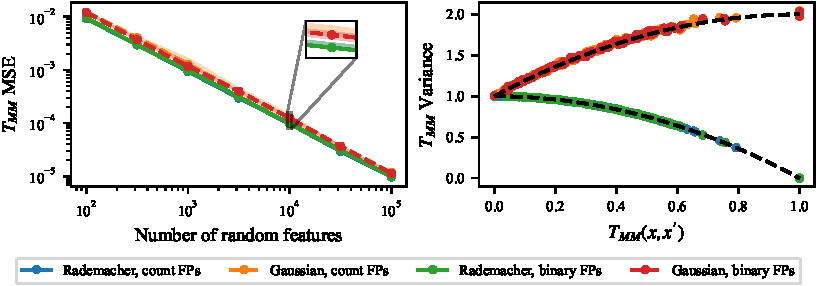
\includegraphics{chapter0x-TRF/new-figures/tmm_variance.pdf}
    \caption[Errors of TMM random features on real data]{
    \textbf{Left:} MSE of $T_{MM}$ matrix reconstruction as a function of number of random features (median over 5 trials, shaded regions are first/third quartiles).
    \textbf{Right:} empirical variance of scalar $T_{MM}$ random feature estimates for $M=10^5$,
    closely matching theoretical predictions (dashed lines).
    }
    \label{fig:tmm-rfs}
\end{figure}

Here we study the error of approximating matrices of Tanimoto coefficients using our random features,
with the general goal of verifying the claims in sections~\ref{sec:minmax-rf}--\ref{sec:t-dp} on a realistic dataset of molecules.
We choose to study a sample of 1000
small organic molecules from the GuacaMol dataset \citep{brown2019guacamol,mendez2019chembl} %
which exemplify the types of molecules typically considered in drug discovery projects.
We use both binary (B) and count (C) fingerprints of radius 2.

First, we investigate the random features for $T_{MM}$ proposed in section~\ref{sec:minmax-rf}.
We instantiate these features using the random hash from \citet{ioffe2010improved} (explained further in Appendix~\ref{apdx:explain tmm features and hash})
with $\Xi$ both Gaussian and Rademacher distributed.
The results are shown in Figure~\ref{fig:tmm-rfs}.
The left subplot shows the median mean squared error (MSE), i.e.
$$\mathbb{E}_{i,j} \left[\left(T_{MM}(x^{(i)}, x^{(j)})-\phi(x^{(i)})\cdot \phi(x^{(j)}) \right)^2\right]$$ as a function of the random feature dimension $M$.
As expected for a Monte Carlo estimator, the square error decreases with $\mathcal O(1/M)$ (i.e.\@ increasing the number of random features by 10 reduces the MSE by a factor of 10).
As predicted by Theorem~\ref{thm:general-minmax-rf},
the estimation error seems to depend only on the distribution of $\Xi$ and not on the input vectors themselves;
therefore the error curves for count and binary fingerprints overlap completely.
The error is lowest when $\Xi$ is Rademacher distributed, although the empirical difference in error seems small.
The right subplot looks at the variance across scalar random features,
showing close matching with the predictions of Theorem~\ref{thm:general-minmax-rf}.
Overall these features behave exactly as expected.

\begin{figure}
    \centering
    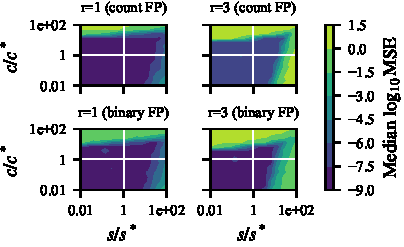
\includegraphics{chapter0x-TRF/new-figures/tdp_prefactor_contours.pdf}
    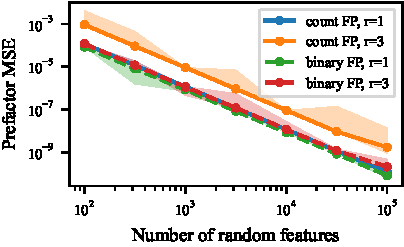
\includegraphics{chapter0x-TRF/new-figures/prefactor_mse.pdf}
    \caption[Errors of TDP prefactor random features on real data.]{
    \textbf{Left:} Contour plots of MSE for prefactor random features with $M=10^4$ with varying $s,c$.
    \textbf{Right:} MSE vs number of prefactor random features with $s,c$ values from \Cref{QMC error}.
    As in Figure~\ref{fig:tmm-rfs}, lines are medians over 5 trials, shaded regions are first/third quartiles.
    }
    \label{fig:prefactor-rfs}
\end{figure}

Next, we investigate the random features for $T_{DP}$ from section~\ref{sec:t-dp}.
These features are more complex, so we start by studying the random features for the ``prefactor''
from section~\ref{ssec:prefactor-rf}.
Recall that these features had free parameters $s,c>0$.
Fixing the number of features $M=10^4$,
Figure~\ref{fig:prefactor-rfs} (left) shows the MSE for the $r=1$ and $r=3$ terms
for both the binary and count fingerprints (which have different norms) as a function of $s$ and $c$.
The values which minimise the relative error bound from \cref{QMC error},
denoted $s^*,c^*$,
seem to lie in a broad plateau of low error in all settings,
suggesting that these values of $s,c$ are a prudent choice.
Using these values of $s,c$,
Figure~\ref{fig:prefactor-rfs} (right) shows the MSE with respect to the number of features $M$.
As expected for a QMC method,
the error dependence appears to be \emph{quadratic} $\mathcal O(1/M^2)$ (i.e.\@ a ten-fold increase in $M$ reduces MSE by 100-fold).


Because it is implemented in \texttt{scikit-learn} \citep{scikit-learn},
we use \textsc{TensorSketch} \citep{pagh2013compressed}
both as the polynomial random feature map and to combine the polynomial and prefactor
random features.
We fix the number of random features for the prefactor to be $10^4$ (recall it can be chosen freely without impacting the final random feature dimension).
Figure~\ref{fig:tdp-polynomial-and-single-term-error} shows the MSE of approximating both $(x\cdot x')^r$
and $((x\cdot x')/(\|x\|^2+\|x'\|^2))^r$.
In both cases, the MSE decreases approximately with $\mathcal O(1/M)$.
Finally, we empirically examine how to allocate $M$ random features across $R$ terms.
Using $R=4$, Figure~\ref{fig:tdp-total-rf} (left) shows that allocating most of the features to the terms with small $R$ results in lower error.
We therefore heuristically suggest allocating features according to $\tilde{m}_r\propto r^{-1}$.
Recall that truncating the power series biases the random features downward,
and in section~\ref{sec:tdp-rf} two bias correction techniques were proposed.
Figure~\ref{fig:tdp-total-rf} (right) studies the overall MSE for the plain features
and both bias correction techniques.
It appears that, in practice, neither technique is particularly helpful (normalization in fact appears harmful for large $M$).
All techniques show an error dependence of approximately $\mathcal O(1/M)$.

\begin{figure}[ht]
    \centering
    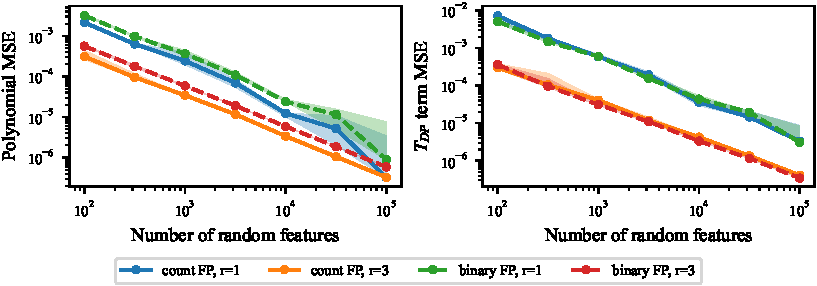
\includegraphics{chapter0x-TRF/new-figures/poly_and_term_term_mse.pdf}
    \caption[Errors of polynomial and single-term random features on real data.]{
        MSEs for approximating $(x\cdot x')^r$ (\textbf{left})
        and $((x\cdot x')/(\|x\|^2+\|x'\|^2))^r$ (\textbf{right})
        using \textsc{TensorSketch} for various $r$ on count and binary fingerprints
        as a function of the random feature dimension $M$.
    }
    \label{fig:tdp-polynomial-and-single-term-error}
\end{figure}


\begin{figure}
    \centering
    {Binary fingerprints} \\
    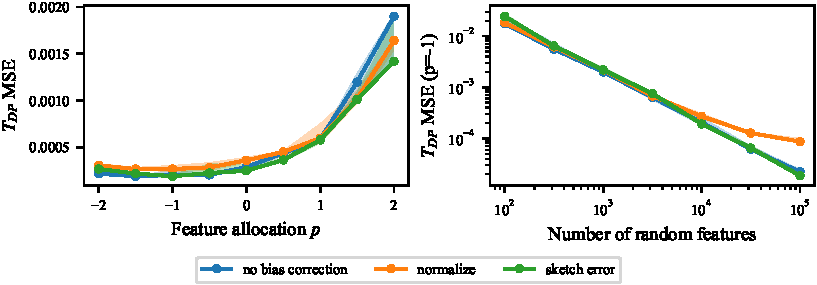
\includegraphics{chapter0x-TRF/new-figures/tdp_feat_alloc_and_overall_error_binary.pdf} \\
    {Count fingerprints}\\
    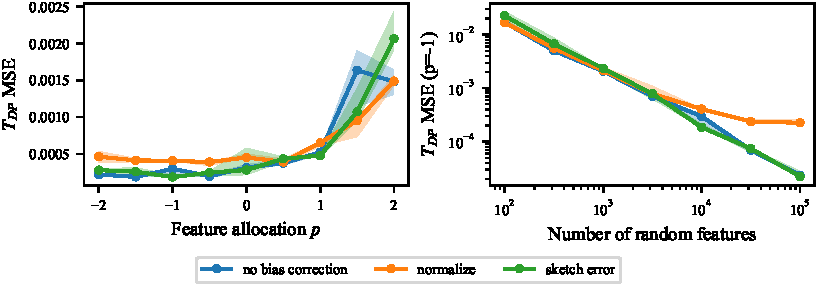
\includegraphics{chapter0x-TRF/new-figures/tdp_feat_alloc_and_overall_error_count.pdf}
    \caption[Errors of TDP random features on real data.]{
    \textbf{Left:} MSE for $M=10^4$ dimensional random features when allocating features by $\tilde{m}_r\propto r^p$, $r=1.\ldots,4$.
    \textbf{Right:}  MSE of $T_{DP}$ random features using $R=4,p=-1$ and various bias correction strategies.
    As in Figure~\ref{fig:tmm-rfs}, lines are medians over 5 trials, shaded regions are first/third quartiles.
    }
    \label{fig:tdp-total-rf}
\end{figure}




\subsection{Molecular property prediction and uncertainty quantification}\label{sec:regression-expt}

To evaluate their efficacy in practice, we use our random features to approximate large-scale Gaussian processes (GPs) \citep{rasmussen2006gp}
for molecular property prediction.
Specifically, we study 5 tasks from the \textsc{dockstring} benchmark 
which entail predicting protein binding affinity from a molecular graph structure \citep{ortegon2021dockstring}.
Each task contains $250\mathrm{k}$ molecules, making exact GP regression infeasible. 
We represent molecules with count Morgan fingerprints of radius 1.

We use $M=5000$ random features for all methods.
We compare to two approximate GP baselines.
The first is an exact GP on a random subset of size $M$.
Since this approach ignores most of the dataset,
one should expect a reasonable approximate GP to perform better.
The second is a sparse variational GP (SVGP) which approximates the dataset using $M$ pseudo-data points $Z$
\citep{titsias2009variational,hensman2013gaussian}.
The locations of $Z$ are typically chosen based on the input dataset (we use K-means clustering),
making this method effectively a data-dependent sketch.
Accordingly, one might expect the performance of this approximation to be \emph{better}
than data-oblivious random features.
Details of Gaussian process training are given in \cref{apdx:regression-expt-details}.

\begin{table*}[tb]
\caption[Average log probabilities of dockstring test set labels with various approximate GPs.]{
Average log probability of test set labels with various approximate GPs
for 5 targets from \textsc{dockstring} dataset \citep{ortegon2021dockstring}.
$\pm$ values are standard deviations over 5 trials.
}
\label{tab:gp-regression-logp}
\begin{center}
\resizebox{0.95\textwidth}{!}{
\begin{sc}
\begin{tabular}
{llr@{\hspace{0.02cm}$\pm$\hspace{0.02cm}}l@{\hspace{0.30cm}}r@{\hspace{0.02cm}$\pm$\hspace{0.02cm}}l@{\hspace{0.30cm}}r@{\hspace{0.02cm}$\pm$\hspace{0.02cm}}l@{\hspace{0.30cm}}r@{\hspace{0.02cm}$\pm$\hspace{0.02cm}}l@{\hspace{0.30cm}}r@{\hspace{0.02cm}$\pm$\hspace{0.02cm}}l@{\hspace{0.30cm}}}
\toprule
Kernel & Method & \multicolumn{2}{c}{ESR2} & \multicolumn{2}{c}{F2} & \multicolumn{2}{c}{KIT} & \multicolumn{2}{c}{PARP1} & \multicolumn{2}{c}{PGR}\\
\midrule
$T_{MM}$ & Rand subset GP & -1.084 & 0.004 & -0.951 & 0.002 & -1.094 & 0.002 & -0.999 & 0.002 & -1.183 & 0.005\\
 & SVGP & -0.908 & 0.005 & -0.502 & 0.005 & -0.846 & 0.002 & -0.606 & 0.005 & -1.030 & 0.005\\
 & RFGP ($\Xi$ Rad.) & -0.954 & 0.009 & -0.658 & 0.013 & -1.222 & 0.044 & -0.968 & 0.037 & -1.127 & 0.023\\
 & RFGP ($\Xi$ Gauss.) & -0.956 & 0.010 & -0.663 & 0.015 & -1.230 & 0.048 & -0.967 & 0.036 & -1.124 & 0.025\\
\midrule
$T_{DP}$ & Rand subset GP & -1.073 & 0.002 & -0.940 & 0.001 & -1.077 & 0.002 & -0.988 & 0.001 & -1.187 & 0.006\\
 & SVGP & -0.880 & 0.004 & -0.459 & 0.002 & -0.804 & 0.002 & -0.568 & 0.002 & -1.010 & 0.004\\
 & RFGP (plain) & -0.902 & 0.003 & -0.513 & 0.004 & -0.979 & 0.015 & -0.690 & 0.022 & -1.029 & 0.002\\
 & RFGP (norm) & -0.902 & 0.003 & -0.515 & 0.003 & -0.980 & 0.015 & -0.691 & 0.022 & -1.028 & 0.002\\
 & RFGP (sketch) & -0.904 & 0.002 & -0.515 & 0.004 & -0.979 & 0.014 & -0.690 & 0.021 & -1.030 & 0.002\\
\bottomrule
\end{tabular}

\end{sc}
}
\end{center}
\end{table*}

Table~\ref{tab:gp-regression-logp} shows the average log probability\footnote{
    Calculated by first calculating the log probability of each test point individually
    (i.e.\@ marginally, not jointly), then averaging these values.
}
of test set labels
for all types of GP with $T_{MM}$ and $T_{DP}$ kernels.
Several trends are evident.
First, for each kernel random feature GPs (RFGPs) consistently outperform random subset GPs,
but underperform SVGP.
Second, for each kernel the difference between the RFGP varieties is small
(generally less than the standard deviation).
Third, on most targets $T_{DP}$ seems to perform better than the $T_{MM}$ kernel.
The reason for this is unclear.

Similar trends can be seen in the $R^2$ metric\footnote{
    This is calculated using the function \texttt{sklearn.metrics.r2\_score}.
    This measures only the error of the GP mean.
    A value of 1 indicates perfect prediction,
    while a value of 0 can be achieved by predicting the sample mean for every data point.
}
in Table~\ref{tab:gp-regression-r2}.
Because $R^2$ only uses point predictions,
we also include baselines for two types of graph neural network:
Attentive FP \citep{xiong2019pushing}
and MPNN \citep{gilmer2017neural}.
Although the performance of GP methods does not match that of Attentive FP,
it is often close,
suggesting there is potential for approximate GPs to be competitive with graph neural networks
for molecular property prediction.

Overall, this suggests that the RFGPs developed in this chapter can be used in large-scale regression,
although it seems in practice that data-dependent approximations are more accurate.

\begin{table*}[tb]
\caption[$R^2$ scores of various approximate GPs on dockstring test set.]{
Average $R^2$ score for approximate GPs on \textsc{dockstring} dataset.
Attentive FP and MPNN results
are taken from \citet{ortegon2021dockstring}.
Other details are the same as Table~\ref{tab:gp-regression-logp}.
}
\label{tab:gp-regression-r2}
\begin{center}
\resizebox{0.95\textwidth}{!}{
\begin{sc}
\begin{tabular}
{llr@{\hspace{0.02cm}$\pm$\hspace{0.02cm}}l@{\hspace{0.30cm}}r@{\hspace{0.02cm}$\pm$\hspace{0.02cm}}l@{\hspace{0.30cm}}r@{\hspace{0.02cm}$\pm$\hspace{0.02cm}}l@{\hspace{0.30cm}}r@{\hspace{0.02cm}$\pm$\hspace{0.02cm}}l@{\hspace{0.30cm}}r@{\hspace{0.02cm}$\pm$\hspace{0.02cm}}l@{\hspace{0.30cm}}}
\toprule
Kernel & Method & \multicolumn{2}{c}{ESR2} & \multicolumn{2}{c}{F2} & \multicolumn{2}{c}{KIT} & \multicolumn{2}{c}{PARP1} & \multicolumn{2}{c}{PGR}\\
\midrule
$T_{MM}$ & Rand subset GP & 0.514 & 0.002 & 0.810 & 0.002 & 0.695 & 0.002 & 0.849 & 0.001 & 0.426 & 0.007\\
 & SVGP & 0.578 & 0.001 & 0.861 & 0.000 & 0.749 & 0.000 & 0.889 & 0.000 & 0.542 & 0.002\\
 & RFGP ($\Xi$ Rad.) & 0.518 & 0.002 & 0.838 & 0.001 & 0.703 & 0.002 & 0.864 & 0.001 & 0.465 & 0.003\\
 & RFGP ($\Xi$ Gauss.) & 0.517 & 0.002 & 0.837 & 0.000 & 0.702 & 0.001 & 0.864 & 0.001 & 0.467 & 0.004\\
\midrule
$T_{DP}$ & Rand subset GP & 0.513 & 0.003 & 0.817 & 0.001 & 0.696 & 0.002 & 0.851 & 0.001 & 0.384 & 0.011\\
 & SVGP & 0.581 & 0.001 & 0.865 & 0.000 & 0.753 & 0.001 & 0.889 & 0.000 & 0.543 & 0.002\\
 & RFGP (plain) & 0.546 & 0.001 & 0.852 & 0.001 & 0.716 & 0.002 & 0.876 & 0.000 & 0.512 & 0.002\\
 & RFGP (norm) & 0.546 & 0.001 & 0.852 & 0.001 & 0.715 & 0.002 & 0.876 & 0.000 & 0.513 & 0.002\\
 & RFGP (sketch) & 0.545 & 0.001 & 0.852 & 0.001 & 0.716 & 0.002 & 0.876 & 0.000 & 0.510 & 0.002\\
\midrule
N/A & MPNN & 0.506 & 0.001  & 0.798 & 0.005  & 0.755 & 0.005  & 0.815 &  0.010 & 0.324 &  0.096 \\
N/A & Attentive FP & 0.627 &  0.010 & 0.880 &  0.001 & 0.806 &  0.008 & 0.910 &  0.002 & 0.678 & 0.008 \\
\bottomrule
\end{tabular}

\end{sc}
}
\end{center}
\end{table*}





\subsection{Bayesian optimisation in molecule space via Thompson sampling}\label{sec:expt-bayesopt}

Bayesian optimisation (BO) uses a probabilistic surrogate model to guide optimisation
and is generally considered one of the most promising techniques for sample-efficient optimisation \citep{shahriari2015taking}.
Because wet-lab experiments are expensive and time-consuming,
there is considerable interest in using BO for experiment design.
Chemistry experiments are often done in large batches,
and therefore algorithms which use functions sampled from a probabilistic model are of particular interest \citep{hernandez2017parallel}.
To sample from a normal distribution $\mathcal{N}(\mu,K)$ one typically transforms i.i.d.\@ samples $Z~\sim\mathcal{N}(0,1)$ via $\mu+K^{1/2}Z$.
This requires computing $K^{1/2}$, and thereby causes exact GP sampling to scale cubically in the number of \emph{evaluation} points.
By approximating $K\approx \Phi^T \Phi$,
our random features allow for approximate sampling in \emph{linear} time.
In this section we apply this to a real-world dataset.

\begin{figure}[h]
    \centering
    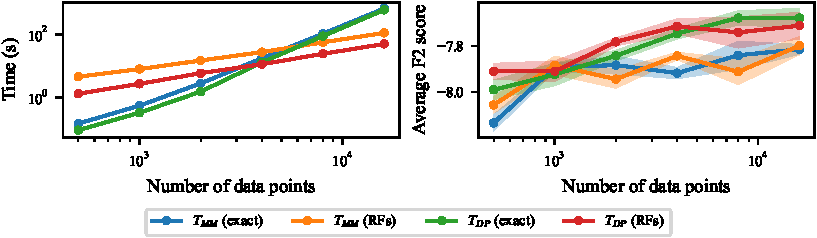
\includegraphics{chapter0x-TRF/new-figures/bo_results.pdf}
    \caption[Results of Bayesian optimisation using exact and approximate Thompson sampling.]{
        Run time and docking scores of BO using exact and approximate Thompson sampling.
        Solid lines are means over 5 trials, shaded regions are standard errors.
    }
    \label{fig:thompson-sampling-results}
\end{figure}

As a demonstration, we consider a single round of selecting 100 molecules from a random sub-sample of $n$ molecules using \emph{Thompson sampling}
(equation~\ref{eqn:backgroun:thompson sampling}) with the $T_{MM}$ and $T_{DP}$ kernels.
Similar to the setup from section~\ref{sec:regression-expt},
we use molecules and labels from the \textsc{dockstring} dataset.
Molecules are represented as count fingerprints.
$M=5000$ random features used, with Rademacher $\Xi$ for $T_{MM}$ and no bias correction for $T_{DP}$.
All other implementation details are the same as in the previous subsection.
Figure~\ref{fig:thompson-sampling-results} (left) shows that,
as expected, exact Thompson sampling scales worse than
approximate Thompson sampling with random features.
Figure~\ref{fig:thompson-sampling-results} (right) shows that using approximate instead of exact Thompson sampling does not seem to change the average F2 docking scores of the molecules chosen.
This suggests that approximate Thompson sampling could fruitfully be applied to large datasets of molecules
in Bayesian optimisation tasks.


\section{Discussion}\label{sec:trf:conclusion}

In this chapter we presented two kinds of random features to estimate Tanimoto kernel matrices:
one based on random hashes and another based on a power series expansion.
To our knowledge, this is the first investigation into random features for the Tanimoto kernel.
We theoretically analyse their approximation quality 
and demonstrate that they can effectively approximate the Tanimoto kernel matrices on
realistic molecular fingerprint data.
In the process we discovered a new Tanimoto-like kernel over all of $\mathbb{R}^d$
which is a promising substitute for the more established $T_{MM}$
on regression and optimisation tasks.

Despite promising theoretical and experimental results, 
our random features do have some limitations.
We found that it was difficult to efficiently vectorize the computation of the random features for $T_{MM}$,
making them undesirably slow to compute.
For $T_{DP}$, we were able to exhibit an error bound on the spectral norm which depends on certain choices for the base sketch and sketch dimensions; however, 
it is unclear whether these choices are optimal in practice.
Nonetheless,
in Appendix~\ref{apdx:proof-of-kernel-rank} we prove that \emph{exact} low-rank factorizations of $T_{MM}$ and $T_{DP}$ kernel matrices are not possible;
this means that follow-up works could reduce but never eliminate the approximation error.

We are most optimistic about the potential of our random features to be applied in Bayesian optimisation,
in particular by enabling scalable approximate sampling from GP posteriors \citep{wilson2020efficiently}.
Although we briefly explored this technique in section~\ref{sec:expt-bayesopt},
in the future it could allow for sample-efficient Bayesian algorithms for complex tasks like Pareto frontier exploration and 
diverse optimisation using the Bayesian algorithm execution framework \citep{neiswanger2021bayesian}.
These tasks are highly relevant to real-world drug discovery and there are scant new methods poised
to solve them in a sample-efficient way.
We hope that the methods presented in this chapter enable impactful, large-scale applications of the Tanimoto kernel and its two extensions in chemoinformatics.





\section{Retrospective and predictions}

The Tanimoto kernel is widely used, and I have spoken to chemists at conferences who have expressed interest in this work.
That being said, for simply making predictions on a large number of molecules
our experiments suggest that inducing point methods are more effective than random features.
I predict this work will primarily be useful in Bayesian optimisation applications
which need approximate posterior samples (e.g.\@ for Thompson sampling).
